\section{Resultados de la Validación Experimental del Sistema DRL}

La validación del sistema de ejercicios basado en Deep Reinforcement Learning se realizó mediante pruebas piloto con estudiantes reales de la Región de Los Ríos, Chile. La muestra estuvo compuesta por 5 estudiantes del Conservatorio de Música de la Universidad Austral de Chile y 23 estudiantes de enseñanza media de la comuna de Corral, totalizando 28 participantes. El período de evaluación tuvo una duración de 28 días consecutivos, durante los cuales los participantes utilizaron la plataforma para resolver ejercicios de teoría musical guiados por el motor DRL, registrando todas las métricas de interacción, progreso y rendimiento generadas por el sistema adaptativo.

\subsection{Evolución del Rendimiento de los Estudiantes en el Sistema DRL}

Se analizaron tres perfiles representativos de desempeño dentro del sistema de ejercicios adaptativos: el estudiante con mejor rendimiento, un estudiante con rendimiento promedio y el estudiante con menor rendimiento. En la Fig.~\ref{fig:rendimiento_ieee} se presenta la evolución del \textit{proficiency} registrada por el motor DRL para estos tres perfiles a lo largo de la resolución de ejercicios, incluyendo la regresión lineal que muestra la tendencia general de mejora impulsada por las recomendaciones personalizadas del agente.

\begin{figure}[H]
    \centering
    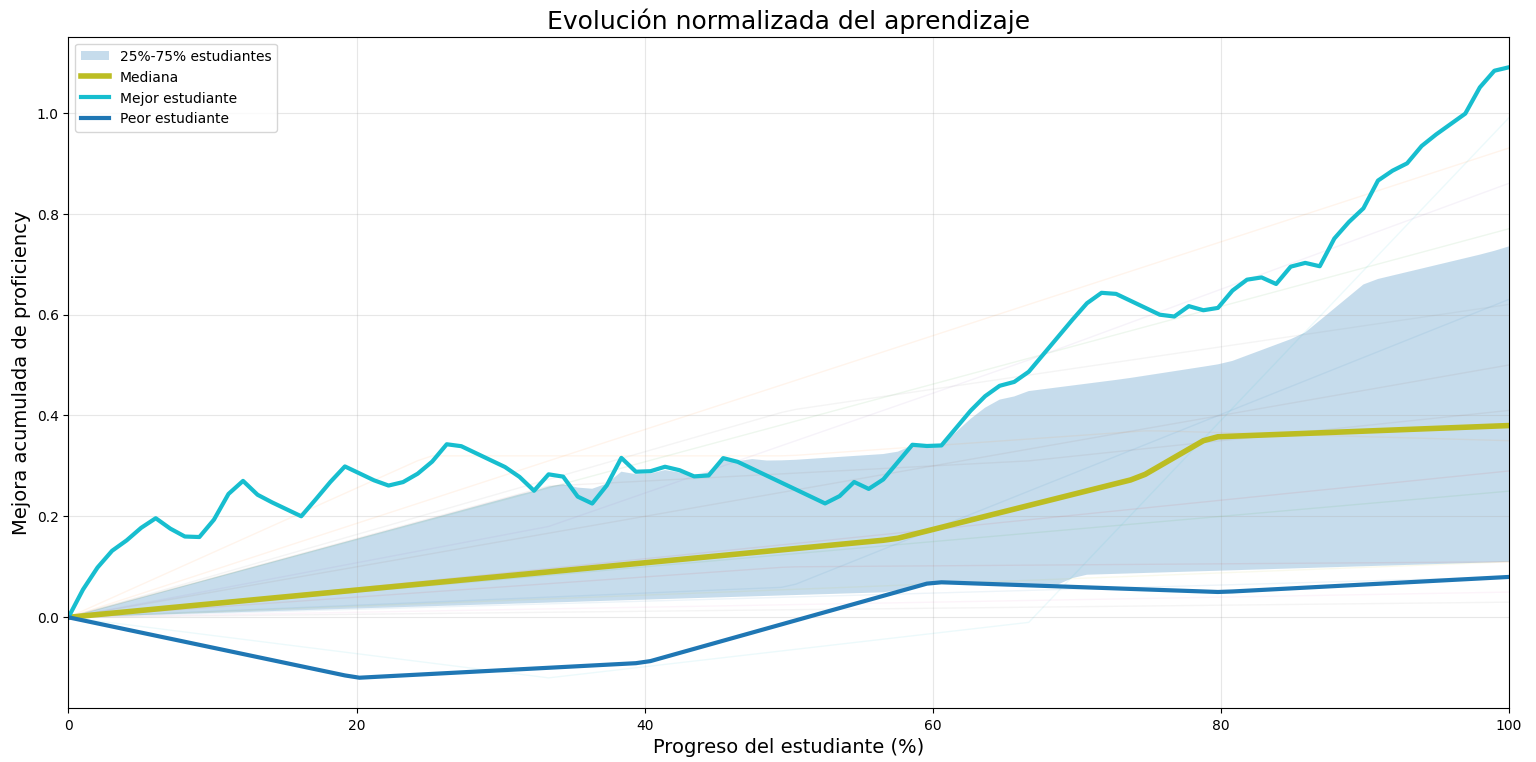
\includegraphics[width=0.49\textwidth]{Imagenes/rendimiento_estudiantes.png}
    \caption{Evolución del rendimiento de los estudiantes durante la validación.}
    \label{fig:rendimiento_ieee}
\end{figure}

Como se observa en el comportamiento del grupo (Fig.~\ref{fig:rendimiento_ieee}), los tres perfiles muestran una tendencia ascendente en su nivel de conocimiento registrado por el sistema DRL. El estudiante con mejor rendimiento partió con una base más sólida y mantuvo un crecimiento consistente. El estudiante promedio refleja el comportamiento típico del grupo, con una mejora gradual pero constante. Incluso el estudiante con menor rendimiento, que inició con proficiencias bajas, logró avanzar progresivamente, lo que demuestra la capacidad del motor DRL para adaptar las recomendaciones a distintos niveles de partida.

\subsection{Actividad de los Estudiantes en la Plataforma DRL}

La Fig.~\ref{fig:actividad_ieee} muestra la distribución de la actividad semanal registrada por el sistema de ejercicios DRL durante las cuatro semanas de pruebas piloto.

\begin{figure}[H]
    \centering
    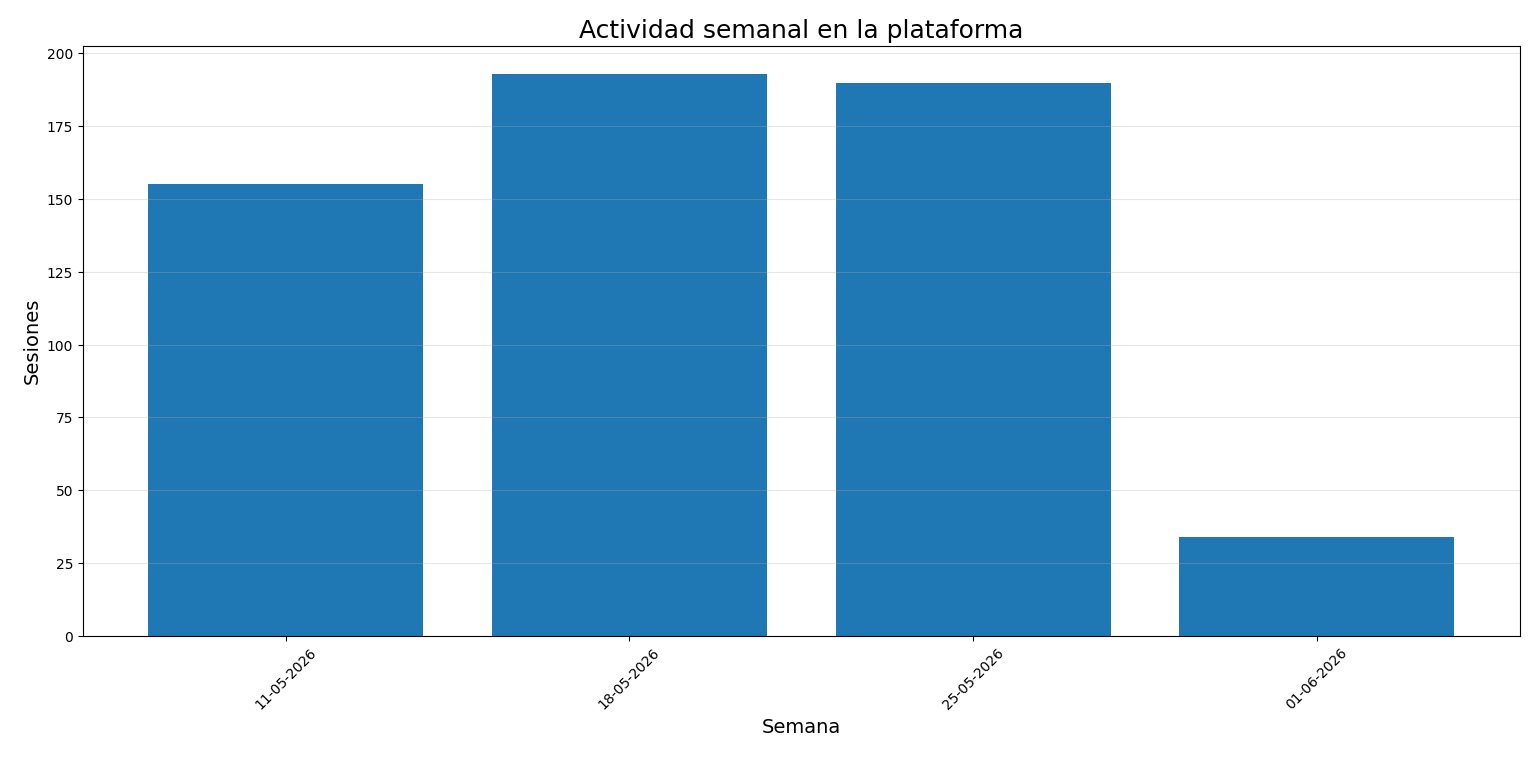
\includegraphics[width=0.49\textwidth]{Imagenes/actividad_semanal.png}
    \caption{Distribución de la actividad por semana durante la fase de pruebas piloto.}
    \label{fig:actividad_ieee}
\end{figure}

Durante el período de evaluación se registraron un total de 572 sesiones de interacción distribuidas en cuatro semanas de análisis. La distribución temporal de la actividad registrada se presenta en la Table~\ref{tab:sesiones_semanales}. Se observa una participación activa y sostenida durante las primeras tres semanas del estudio, con valores superiores a 150 sesiones semanales. En la semana del 01 de junio de 2026 se aprecia una disminución en el número de sesiones registradas; sin embargo, este comportamiento no corresponde a una reducción en el interés de los usuarios ni a un abandono de la aplicación. Esta variación se explica por un factor de truncamiento temporal en la recolección de datos, debido a que la extracción de la muestra finalizó a inicios de dicha semana, considerando únicamente los primeros días de actividad y no una semana completa.

\begin{table}[ht]
\centering
\caption{Distribución semanal de sesiones registradas durante el período de evaluación.}
\label{tab:sesiones_semanales}
\begin{tabular}{lc}
\hline
\textbf{Semana} & \textbf{Número de sesiones} \\
\hline
11-05-2026 & 155 \\
18-05-2026 & 193 \\
25-05-2026 & 190 \\
01-06-2026 & 34 \\
\hline
\textbf{Total} & \textbf{572} \\
\hline
\end{tabular}
\end{table}
\subsection{Métricas Generales del Sistema de Ejercicios DRL}

La Table~\ref{tab:resultados_ieee} presenta un resumen de las principales métricas obtenidas por el sistema de ejercicios basado en DRL durante los 28 días de evaluación.

\begin{table}[H]
    \centering
    \caption{Métricas generales del sistema de ejercicios basado en DRL durante la validación.}
    \label{tab:resultados_ieee}
    \begin{tabular}{|p{3.0cm}|p{4.5cm}|}
        \hline
        \textbf{Aspecto evaluado} & \textbf{Resultado observado} \\
        \hline
        Participación de estudiantes & Los 28 estudiantes participantes utilizaron la plataforma durante el período de validación. \\
        \hline
        Continuidad de uso & Se registró actividad de forma sostenida a lo largo de las semanas evaluadas. \\
        \hline
        Interacción con el sistema DRL & Los estudiantes resolvieron ejercicios y avanzaron progresivamente dentro del árbol de conocimiento guiados por las recomendaciones del motor DRL. \\
        \hline
        Progreso en el aprendizaje & La mediana de los estudiantes alcanzó una mejora aproximada del 20\% en su nivel de \textit{proficiency}, superando el objetivo del 15\%. \\
        \hline
        Adaptación del contenido & El sistema DRL ajustó dinámicamente la dificultad y secuencia de los ejercicios según el desempeño individual de cada usuario. \\
        \hline
    \end{tabular}
\end{table}

Las métricas obtenidas por el sistema de ejercicios DRL evidencian que la plataforma logró mantener una participación constante de los estudiantes durante el período de evaluación. La mejora observada en los niveles de \textit{proficiency}, registrada y calculada por el motor DRL, indica que los estudiantes fueron capaces de adquirir nuevos conocimientos a medida que avanzaban dentro del árbol de aprendizaje, lo que sugiere que la estrategia de personalización implementada por el agente de Deep Reinforcement Learning permitió adaptar el contenido a las necesidades de cada usuario, favoreciendo un avance progresivo en los distintos conceptos de teoría musical.